\setcounter{figure}{0}

\section{21st May 2023: Samaria and to the ends of the earth}
\subsection*{Text: Acts 8:25-40}
  \begin{quote}
    [25] Now when they had testified and spoken the word of the Lord, they
    returned to Jerusalem, preaching the gospel to many villages of the
    Samaritans.

    [26] Now an angel of the Lord said to Philip, “Rise and go toward the
    south to the road that goes down from Jerusalem to Gaza.” This is a
    desert place. [27] And he rose and went. And there was an Ethiopian, a
    eunuch, a court official of Candace, queen of the Ethiopians, who was in
    charge of all her treasure. He had come to Jerusalem to worship [28] and
    was returning, seated in his chariot, and he was reading the prophet
    Isaiah. [29] And the Spirit said to Philip, “Go over and join this
    chariot.” [30] So Philip ran to him and heard him reading Isaiah the
    prophet and asked, “Do you understand what you are reading?” [31] And he
    said, “How can I, unless someone guides me?” And he invited Philip to
    come up and sit with him. [32] Now the passage of the Scripture that he
    was reading was this:

    “Like a sheep he was led to the slaughter
        and like a lamb before its shearer is silent,
        so he opens not his mouth.
    [33] In his humiliation justice was denied him.
        Who can describe his generation?
    For his life is taken away from the earth.”


    [34] And the eunuch said to Philip, “About whom, I ask you, does the
    prophet say this, about himself or about someone else?” [35] Then Philip
    opened his mouth, and beginning with this Scripture he told him the good
    news about Jesus. [36] And as they were going along the road they came to
    some water, and the eunuch said, “See, here is water! What prevents me
    from being baptized?” [38] And he commanded the chariot to stop, and they
    both went down into the water, Philip and the eunuch, and he baptized
    him. [39] And when they came up out of the water, the Spirit of the Lord
    carried Philip away, and the eunuch saw him no more, and went on his way
    rejoicing. [40] But Philip found himself at Azotus, and as he passed
    through he preached the gospel to all the towns until he came to
    Caesarea.
  \end{quote}
\subsection*{Notes}
\begin{itemize}
  \item{In our lives, there would be people who we think that don't deserve
  to go to heaven. Such as people like Hitler, rapists, pedophiles, etc.
  Sometimes we think that these people don't deserve to hear the gospel,
  because what if they believe and repent and are forgiven? Or what if it is
  someone who has hurt us deeply?}
  \item{For us, have we erected imaginary walls in our head that prevent us
  from reaching our to particular people groups? A mental exercise: when we
  hear of place names like ``golden mile complex'', ``tekka market'',
  ``geylang'' are there immediately certain people groups that we think of?
  Do we treat those people groups as the ``other''? Sometimes we might
  ``other'' people groups based on race, language, socioeconomic class, etc.
  This is even more clearly seen in the covid pandemic. In the pandemic, we
  see a systemic difference between Singaporeans and the migrant workers; the
  treatment for these two people groups were very different.}
  \item{Sometimes,these walls even exist in our church groups, that's why we
  form cliques. We form cliques based on people who think, speak or act like
  us. }
  \item{Yet when we read the gospel accounts, in Jesus' ministry, we see that
  He was more interested in breaking down walls and building bridges. For
  example, Jews usually do not talk to Samaritans, but we see Jesus
  intentionally speaking to the Samaritan woman at the well. We also should
  consider Jesus' ministry to the poor, the tax collectors, and the
  prostitutes. And at Jesus' ascension, we remember Jesus' words to take the
  gospel to Samaria and to the end of the world.}
  \item{In our text, we see the Spirit directing Philip to Samaria, to
  minister to the Ethiopian eunuch. In OT times, Ethiopia was known as Cush.
  And in OT times, Cush was considered ``the ends of the world'', since
  Israel didn't have a globe or Wikipedia lol. Here we see how Philip
  transcending the barriers that might have divided them; the Ethiopian was
  dark skinned, Philip was probably not as dark. The Ethiopian was rich,
  Philip wasn't. We can see how wealthy the Ethiopian was by the fact that he
  had his own chariot and he had hs own scroll of Isaiah.}
  \item{Lastly, this Ethiopian was a enunuch (c.f Isaiah 56), but not Philip.
  This eunuch was probably a proselyte (convert to Judaism), since he was
  returning to Ethiopia from Jerusalem (v27). Note that in OT times, at least
  based on the Deuteronomic prohibition on who can enter into the assembly of
  the LORD, the eunuch was probably stuck in the court of the Gentiles (the
  outer courtyard) in the Temple. This makes the passage in Isaiah that he
  was reading from even more significant. Since Isaiah is a large book, in
  olden days, it was split across multiple scrolls. The part that the eunuch
  was reading from is categorised as what is known as the ``fourth servant
  song'', which starts from Isaiah 53. Since he was reading from the ``fourth
  servant song'', he would also have read Isaiah 56. }
  \item{This background makes the eunuch's question even more piercing. The
  eunuch asked: ``is there any reason why I cannot be baptised?''. At least
  from the OT perspective, he couldn't have enterted into the assembly of the
  LORD. But here we see the difference between the NT perspective and the OT
  perspective in Deuteronomy. We see how Philip tore down the walls of
  division that separated people groups, such as the wall between the Jews
  and Gentiles. This is exactly what was mentioned in Ephesians 2:14-18. In
  the baptism of this Eunuch, Philip was fulfilling in Isaiah 56 that even
  all the Gentiles and the eunuchs can be counted as God's covenant people.}
  \item{Now, we note that all of this was before Peter met Cornelius, and
  before Paul was commissioned as an apostle to the Gentiles.}
  \item{What then, is the lesson for us? One lesson is that God feels
  passionately for the people on the other side of the wall that WE have
  erected in keeping them out. Again, from Ephesians 2:14-18, we see how God
  is creating a new people, a people undivided by ethnicity, by socioeconomic
  class, etc etc. Or again, in Galatians, ``there is no male or female, Jew
  or Greek, slave and free''. What binds all these diverse people groups is
  God's love for every single people group and our love for Jesus. Only Jesus
  is the one that can bring about healing and transformation and forgiveness,
  and that is true for all peoples.}
  \item{And one symbol of this Christian unity is the Lord's supper (c.f 1
  Corinthians 10:17, ``Because there is one bread, we who are many are one
  body, for we all partake of the one bread.''). }
  \item{In our ministry, even when we are reaching out to those who are
  considered as the ``other'', we should not stay in our comfort zone and
  wait for the ``other'' to come to us, we should GO into where the ``other''
  are! An example is Healthserve; when Dr Goh started his clinic, there
  weren't many people who came, until he went to where the migrant workers
  were!}
  \item{Our Christian faith, our evangelism (especially in SG), cannot be
  ethnocentric. We cannot just reach out to the people who are the same as
  us! Are we erecting walls that divide, or are we building bridges?}
  \item{\begin{figure}[H]
    \centering
    % 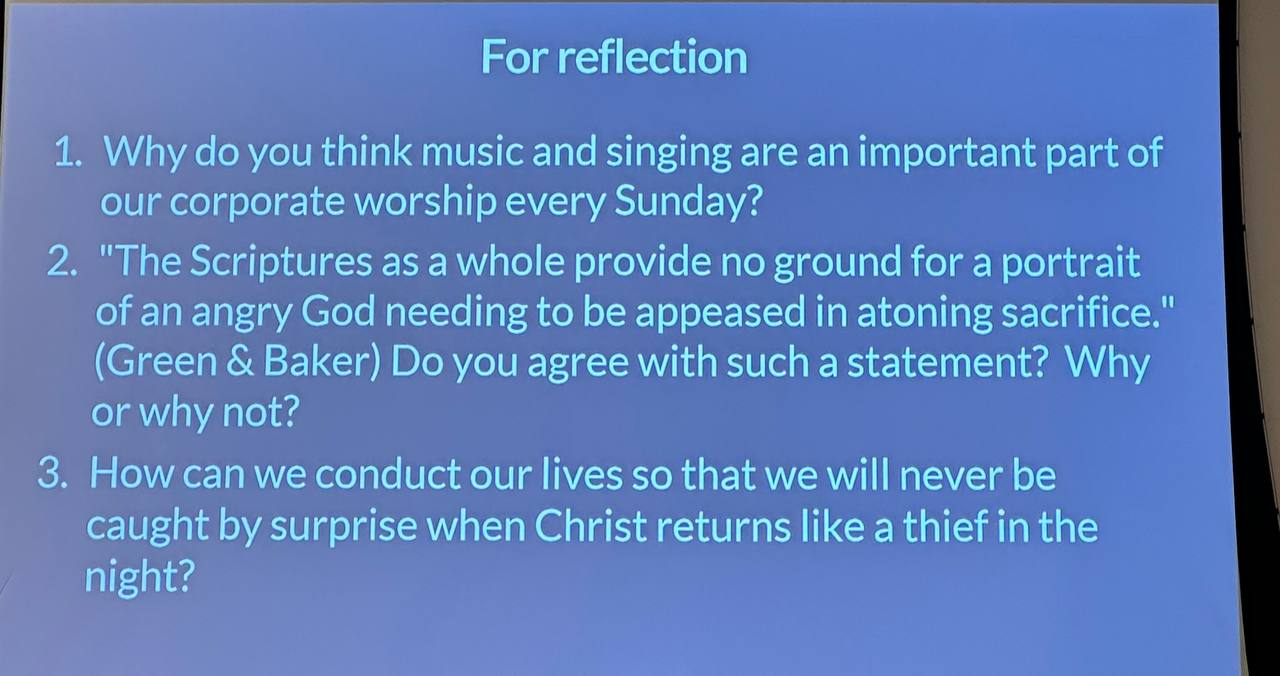
\includegraphics[width=0.8\textwidth, trim={0cm 0cm 0cm 0cm},clip]{Figures/marchSermon4Reflections.jpg}
    \includegraphics[width=0.8\textwidth, trim={0cm 0cm 0cm 0cm},clip]{example-image-a}
    \caption[]{Reflection questions for this sermon}
    % \label{}
  \end{figure}}
\end{itemize}